% *** LaTeX-mal for labrapporter i fysikk, v.14.08.2017 ***

% Dette er et eksempel på et LaTeX-dokument, og du kan bruke dette som et utgangspunkt for din egen rapport. Merk at for å kunne kompilere dokumentet uten feil, må du også laste ned filen pendel-oppdatert.pdf.
%
% Her i starten og videre nedover i teksten under har vi lagt inn en god del linjer som starter med tegnet "%". Disse linjene er kommentarer og synes ikke i det ferdige dokumentet. Vi kan også sette inn et kommentartegn midt på en linje. Alt som kommer før tegnet brukes da i kompileringen, mens resten av linja er en kommentar. 
%
% Kildefilen (.tex-filen) begynner alltid med et "preabmle". Her setter man opp innstillingene som brukes av kompilatoren til å utforme det ferdige dokumentet. Selve dokumentet begynner ikke før vi skriver \begin{document}.
%
% Dokumentasjon for alle pakker finnes på CTAN (http://www.ctan.org/)

%%%%%%%%%%%%%%%%%%%%%%%%%%%%%%%%%%%%%
% Preamble
%%%%%%%%%%%%%%%%%%%%%%%%%%%%%%%%%%%%%

\documentclass[5p,sort&compress]{elsarticle}		
% 5p gir 2 kolonner pr side. 1p gir 1 kolonne pr side.
% Valget sort&compress gjør at referansen [1,2,3] settes som [1-3]. 
% Andre innstillinger for "klassen" elsarticle finnes i dokumentasjonen på CTAN (http://www.ctan.org/pkg/elsarticle)

% Klassen elsarticle er laget for bruk i engelskspråklige tiksskrift. I blokken under bruker vi litt lavnivå TeX-magi for å redefinere bunnteksten på tittelsiden. Ikke bekymre deg for denne biten med kode, det som kommer lengere nede i dokumentet er lettere å forstå!
\makeatletter
\def\ps@pprintTitle{%
 \let\@oddhead\@empty
 \let\@evenhead\@empty
 \def\@oddfoot{\footnotesize\itshape
       Utkast levert til Veileder	% Bytt ut "Veileder" med navnet på veilederen din!
       \hfill\today}%
 \let\@evenfoot\@oddfoot}
\makeatother

% Encoding for input i tex-filen og encoding for output i pdf-filen
\usepackage[utf8]{inputenc}
\usepackage[T1]{fontenc}
\usepackage{textcomp}

% Last inn en font-pakke. Her bruker vi standard-fonten til LaTeX. 
\usepackage{lmodern}

% LaTeX gjør mye av typografien for deg, blant annet orddeling ved linjeskift og automatisk utfylling av endel tekst. For å kunne gjøre dette må kompilatoren vite hvilket språk dokumentet er skrevet på. 
\usepackage[norsk]{babel}
\usepackage[fixlanguage]{babelbib}
% Til tross for at vi har fortalt kompilatoren at vi skriver på norsk må vi fortelle den eksplisitt at vi ønsker at seksjonen "abstract" skal kalles "sammendrag"
\renewenvironment{abstract}{\global\setbox\absbox=\vbox\bgroup
\hsize=\textwidth\def\baselinestretch{1}%
\noindent\unskip\textbf{Sammendrag}
\par\medskip\noindent\unskip\ignorespaces}
{\egroup}

% Mikrotypografiske optimeringer
\usepackage[babel=true]{microtype}

% AMS-utvidelsene for å håndtere matematikk
\usepackage{amsmath}
\usepackage{amssymb}
\usepackage{bm}

% Måltall og enheter er spesielle typografiske dyr som reguleres av strenge regler. For å gjøre det enklere å håndtere tall og enheter på riktig måte bruker vi pakken siunitx.
\usepackage{siunitx}
% Vi tilpasser standardinstillingene til pakken til norske regler. 
\sisetup{
exponent-product = \cdot,
output-decimal-marker  =  {,}, % Pass på å endre desimalskilletegnet til punktum om du skriver på engelsk!
separate-uncertainty = true,
per-mode = symbol,
group-digits = false,
}

% Figurer og tabeller
\usepackage{graphicx} % Denne pakken er standard for å kunne laste inn figurfiler med ulike formater
% Løsne opp på de alt for strenge standardinstillingene for plassering av figurer og tabeller (floats) i LaTeX-kjernen
\renewcommand{\topfraction}{.85}
\renewcommand{\bottomfraction}{.7}
\renewcommand{\textfraction}{.15}
\renewcommand{\floatpagefraction}{.66}
\setcounter{topnumber}{3}
\setcounter{bottomnumber}{2}
\setcounter{totalnumber}{10}
\usepackage{flafter} % For å plassere floats i PDFen første sted LaTeX tillater etter det punktet de er definert i TeX-filen. Om du definerer figuren i TeX-filen rett etter at du refererer til den for første gang vil denne pakken sørge for at de fleste floats havner på greie steder
\usepackage{booktabs} % Denne pakken gir tilgang på endel ekstra kommandoer som legger til rette for god skikk og bruk i tabellformatering.
\usepackage{multirow}
\usepackage[font=small,labelfont=bf]{caption}	% Justering av LaTeX standarder for figurtekst og tabelltekst.

% Hyperreferanser
\usepackage[colorlinks=true,allcolors=blue]{hyperref}
% Noen av navnene for autoreferanser mangler på norsk, så vi ordner opp i det.
\addto\extrasnorsk{%
\def\figureautorefname{figur}%
\def\tableautorefname{tabell}%
\def\sectionautorefname{avsnitt}%
\def\subsectionautorefname{underavsnitt}%
\def\equationautorefname~#1\null{ligning~(#1)\null}
}
% Vi endrer fonten som brukes for URLer til den vanlige tekstfonten.
\urlstyle{same}

%%%%%%%%%%%%%%%%%%%%%%%%%%%%%%%%%%%%%
% Selve dokumentet
%%%%%%%%%%%%%%%%%%%%%%%%%%%%%%%%%%%%%

\begin{document}

% I "front matter" angir vi formalia knyttet til dokumentet -- tittel, forfatter, tilknytning og sammendrag
\begin{frontmatter}

\title{Mal for rapport til laboratorium i fysikk}

% I forfatterlisten legger vi inn "ikke-brytende" mellomrom etter initialene
\author{J.~O.~Bruun}
\author{S.~Klyve}

\begin{abstract}
Sammendraget er en kort og konsis oppsummering av innholdet i rapporten. Sammendraget er den delen av rapporten som skal skrives sist, når du har full kontroll på alt innholdet. En god lengde for et sammendrag er 4--5 setninger. I løpet av disse setningene skal forsøket introduseres, du skal fortelle hvilke metoder som ble brukt, resultatene skal presenteres og du må fortelle kort hva resultatene betyr. Om resultatet eksisterer i form av et tallsvar skal dette oppgis med tilhørende usikkerhet. 
\end{abstract}

\end{frontmatter}


\section{Introduksjon}
Stefan-Boltzmanns lov er en viktig relasjon i fysikken, som forbinder emittert varmeenergi  fra et svart legeme, med dets temperatur. Den ble først formulert av Joseph Stefan i 1879, og utledet av Ludwig Boltzmann fem år senere (INSERT KILDE). I dette forsøket skal vi studere emissiviteten til ulike overflater ved ulike temperaturer, i tillegg til å verifisere Stefan-Boltzmanns lov ved å sjekke forholdet mellom temperatur og emittert varme fra et objekt.


Her begynner den egentlige rapporten. Mer informasjon om hva de enkelte delene av rapporten skal inneholde finnes på nettsiden til laben~\cite{labside}. På slutten av forrige setning ser vi et eksempel på en referanse. Her er et eksempel på en referanse til læreboka~\cite{Young2016}. Referanselisten kommer til slutt i rapporten. I denne malen har vi brukt \textsc{Bib}\TeX\ til å formatere referansene, men det er også mulig å formatere dem manuelt direkte i \texttt{tex}-filen. 
% BibTeX er det programmet som tradisjonelt brukes til automatisert referansehåndtering i LaTeX. Den mest moderne måten å håndtere referanser på er pakken biblatex, men den kan ikke brukes sammen med elsarticle.



\section{Teori}
Et svart legeme er et objekt som absorberer all innkommende strålingsenergi, uavhengig av bølgelengden. Dersom objektet er i termisk likevekt, blir det totalt sett hverken tilført eller avgitt energi. Det vil si at objektet må emittere like mye stråling som det absorberer for å oppnå likevekt. For et svart legeme betyr dette at den emitterte strålingsenergien er lik den absorberte. Forholdet mellom den emitterte effekten per flateenhet, $j$, og det svarte legemets temperatur er gitt ved Stefan-Boltzmanns lov:

\begin{equation}
  j = \sigma T^4
\label{eq:SB} % Merkelappen til ligningen er det navnet vi bruker når vi skal referere til ligningen senere.
\end{equation}

Her er $\sigma = \SI{5,67e-8}{\watt\metre^{-2}\kelvin^{-4}}$ Stefan-Boltzmann-konstanten. Dersom dette skal gjelde for et objekt med vilkårlig emissivitet $\epsilon$, må vi justere til

\begin{equation}
  j = \epsilon\sigma T^4.
\label{eq:SBepsilon} % Merkelappen til ligningen er det navnet vi bruker når vi skal referere til ligningen senere.
\end{equation}

For å måle temperaturen til glødetråden i en Stefan-Boltzmann-lampe, kan følgende relasjon brukes:

\begin{equation}
  T=T_0+\frac{R-R_0}{\alpha R_0}
\label{eq:TempMetall} 
\end{equation}

Her er $\alpha=\SI{4,5e-3}{\kelvin^{-1}}$ temperaturkoeffisienten til wolfram. $R_0$ er motstanden ved referansetemperatur $T_0$, og $R=\frac{V}{I}$ er motstand ved temperatur $T$. Siden denne relasjonen i utgangspunktet gjelder kun for små temperaturvariasjoner i metallet, må vi bruke relativ motstand $R/R_0$, og lese av temperaturen til wolframtråden fra tabell. Fra dette finner vi usikkerheten i den relative resistansen ved Gauss feilforplantning

\begin{equation}
  \label{eq:ErrorRelRes}
  \left( \Delta \frac{R}{R_{0}} \right) ^{2} = \frac{\Delta R^{2}}{R_{0}^{2}} + \frac{R^{2} \Delta R_{0}^{2}}{R_{0}^{4}}.
\end{equation}

En Wheatstonebro kan brukes til å måle nøyaktig motstand i en krets. Ved bruk av Kirchhoffs lover i lag med flere resistorer, kan unøyaktigheten i målingen presses ned mot veldig lav feilmargin. Dette passer fint til måling av motstanden i Stefan-Boltzmann-lampenved romtemperatur, spesielt med tanke på at feilmarginen i denne målingen vil forplante seg betydlig i resultatene. Feilmarginen i $R_{0}$ kan da finnes ved Gauss feilforplantning
\begin{align}
  \label{eq:ErrorBridge}
  \Delta R_{0}^{2} =& \frac{(R_{x1} - R_{x0})^{2}}{R_{1}^{2}} \left( \Delta R_{3}^{2} + \frac{R_{3}^{2} \Delta R_{1}^{2}}{R_{1}^{2}} \right) \notag \\
  &+ \frac{R_{3}^{2}}{R_{1}^{2}} \left( \Delta R_{x1}^{2} + \Delta R_{x0}^{2} \right).
\end{align}



\section{Metode}
Dette forsøket omfatter i hovedsak to ulike deler; først å undersøke emissivitet til ulike overflater ved ulike temperaturer ved bruk av en Leslies kube, og deretter verifisere Stefan-Boltzmann lov ved å måle emittert varmestråling fra en lampe ved varme temperaturer.

Leslies kube er et objekt med fire ulike overflater; svart, hvit, upolert aluminium og blankt aluminium (speil). Den varmes opp innvendig ved hjelp av en glødepære, og temperaturen til kuben kan leses av i tabell basert på resistansen i en innebygd termistor. Når resistansen stabiliserer seg på en gitt verdi, har kuben oppnådd termostatisk likevekt. Fra dette kan det måles avgitt varmestråling med en strålingssensor, og med det undersøke hvordan dette avhenger med overflate og temperatur.

\begin{figure}
  \centering
  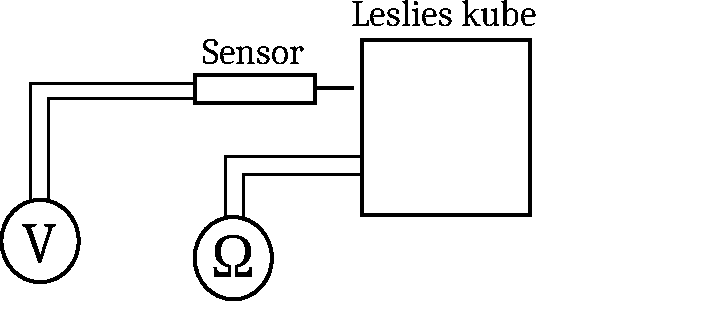
\includegraphics[width=0.4\textwidth]{figures/leslikube.pdf}
  \caption{Utstyrsoppsett. Leslies kube er koblet til et strømuttak og et ohmmeter, varmestrålingssensoren er koblet til et voltemeter.}
  \label{fig:Leslikube}
\end{figure}

For Leslies kube kobles utstyret opp som vist i \autoref{fig:Leslikube} og skrur på lampen i Leslies kuben på høy intesitet først før den skrus ned når ohmmeteteret viser omtrent $\SI{40}{\kilo\ohm}$ før intensiteten skrus ned. Venter så til det oppnås en form for termisk likevekt og måler så varmestråling ved å lese av voltmeteret koblet til sensoren på hver av de fire sidene og skrur så opp intensiteten, venter i omtrent fem minutter til det er tilnærmet termisk likevekt og måler så varmestråling på nytt. Gjør dette fire ganger.

\begin{figure}
  \centering
  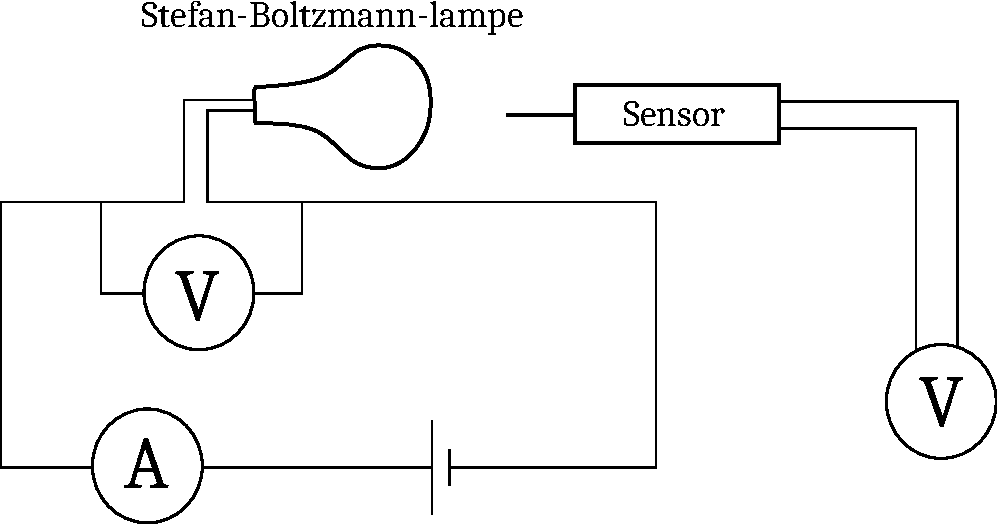
\includegraphics[width=0.4\textwidth]{figures/lampe.pdf}
  \caption{Utstyrsoppsett. Kobler et voltmeter paralelt med Stefan-Boltzmann-lampen i en krets med et ammeter og en spenningskilde som kobles til et strømuttak. Kobler et voltmeter til sensoren.}
  \label{fig:SBlampe}
\end{figure}

Kobler opp utstyr som vist i \autoref{fig:SBlampe}. Setter spenningen til $\SI{1}{\volt}$ og måler så av strøm og spenning i kretsen med Stefan-Boltzmann-lampen og spenningen i varmestrålingssensoren. Setter så opp spenningen med $\SI{1}{\volt}$ og gjør det samme til og med $\SI{12}{\volt}$.


\section{Resultater}
Ofte vil vi skrive inn enkeltmålinger i resultatdelen. Da er det viktig å angi usikkerhet. For eksempel kan lengden til pendelen være $l=\SI{1000,015(5)}{\milli\metre}$. 
% Her har vi brukt kommandoen \SI fra siunitx-pakken for å presentere måltall og enheter på en typografisk korrekt måte. Til tall uten enhet trenger vi en kommando med bare ett argument --  da bruker vi \num{<tall>}. Om vi skal oppgi en enhet uten et måltall bruker vi \si{<enhet>}. Søk opp "siunitx" på CTAN for flere detaljer.
% Legg spesielt merke til hvordan man skriver usikkerheten, og hvordan denne kommer frem i den kompilerte pdfen. 
Vi kan også skrive opp usikkerheten separat. I dette tilfellet har vi $\Delta l=\SI{5e-3}{\milli\metre}$. Alternativt kunne vi skrevet denne usikkerheten som $\Delta l=\SI{5e-6}{\metre}$ eller $\Delta l=\SI{5}{\micro\metre}$.

I resultatdelen er det ofte bruk for tabeller for å presentere måledata på en oversiktlig måte. Husk at alle måledata skal oppgis med usikkerhet! Tabell \ref{tab:ckolonner} er et godt eksempel. 
% Merk at vi ikke brukte \autoref i begynnelsen av setningen fordi vi trengte stor forbokstav. 
I \autoref{tab:Skolonner} ser vi et eksempel der den samme tabellen er laget på en litt annen måte. Merk at mens figurtekster står under figurene skal tabelltekster plasseres over tabellene.

% Tabeller i LaTeX kan være litt vanskelig å forstå, men om du studerer eksemplene nøye blir ting forhåpentligvis litt klarere. Det viktigste du må huske på er at tabellene skrives rad for rad. Ampersand angir skiller mellom kolonner, og \\ angir slutten på raden
\begin{table}[tbp]
\centering % Denne kommandoen sentrerer tabellen i kolonnen. 
\caption{Dette er den obligatoriske tabellteksten. Den kommer over tabellen. Husk at de samme reglene gjelder for utforming av tabellteksten som for utforming av figurteksten.}
\label{tab:ckolonner}	% Merkelappen vi vil referere til.
\begin{tabular}{cc} % Her angir det andre argumentet at vi vil ha to senterjusterte kolonner (l = left, c = center, r = right).
\toprule % Horisontal linje som markerer toppen av tabellen
$h$ [\si{\centi\metre}] & $g$ [\si{\metre\per\second\squared}] \\ % Merk at vi skriver variabelnavnene i kursiv. Det er fordi de er matematiske symboler, og har ingenting med at dette er kolonneoverskrifter å gjøre!
\midrule
20  & 9,836\,$\pm$\,0,004 \\ % Kommandoen \, gir et kort mellomrom.
23  & 9,847\,$\pm$\,0,002 \\
29  & 9,839\,$\pm$\,0,008 \\
33  & 9,840\,$\pm$\,0,001 \\
40  & 9,829\,$\pm$\,0,006 \\
\bottomrule
\end{tabular}
\end{table}
% Formatet på denne tabellen er beskrevet i "Retningslinjer for rapportskriving".

% Tabeller med numerisk data skal være linjert på desimalskilletegnet. Ofte kan dette være vanskelig med en enkel c, l eller r. Her kommer heldigvis pakken siunitx til hjelp med det spesielle kolonneformatet S, som vi skal se i denne neste tabellen. 
\begin{table}[tbp]
\centering
\caption{Denne tabellen har identisk innhold som den forrige, men er laget på en litt annen måte.}
\label{tab:Skolonner}
\begin{tabular}{SS[table-format=1.3(1)]} % S = spesielt kolonneformat håndtert av siunitx.
\toprule
{$h$ [\si{\centi\metre}]} & {$g$ [\si{\metre\per\second\squared}]} \\
% Merk deg at kolonneoverskriftene er omsluttet av krøllparanteser i kolonneformatet S!
\midrule
20  & 9,836(4) \\
23  & 9,847(2) \\
29  & 9,839(8) \\
33  & 9,840(1) \\
40  & 9,829(6) \\
\bottomrule
\end{tabular}
\end{table}

Selv om tabeller er hendige, er de ikke alltid den beste løsningen i resultatdelen. Det er for eksempel lettere å se om det er en sammenheng mellom avstanden fra opphengspunktet til massesenteret og verdien og usikkerheten som ble målt for tyngdeakselerasjonen dersom vi plotter resultatene i en figur. Figur \ref{fig:resultater} er et eksempel på dette. Denne presentasjonsformen blir mer aktuell dersom vi har mange resultater. 

\begin{figure}[tbp]
\centering
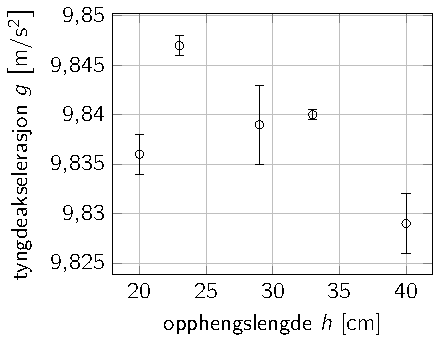
\includegraphics[width=.325\textwidth]{resultater.pdf}
\caption{Denne presentasjonsformen egner seg bedre til å tydeliggjøre trender i datagrunnlaget. Her kan det se ut som om verdien vi måler for $g$ og usikkerheten i målingene er relativt uavhengig av $h$.}
\label{fig:resultater}
\end{figure}

% Figurene og tabellene vi har brukt så langt har vært avgrenset til én kolonnebredde. Om vi trenger tabeller eller figurer som dekker hele sidebredden får vi det ved å bruke miljøene figure* og table*. 

\section{Diskusjon}
Rapportskriving i \LaTeX\ gir mange muligheter. Selv om det er endel tekniske finesser som skal på plass er det viktig å huske på at god skriving og godt språk ligger til grunn for å skrive en god rapport. 

\section{Konklusjon}
Nå har vi gitt endel eksempler på formatering. For å mestre \LaTeX\ er det bare én ting som gjelder -- trening. Last ned kildefilene og lek med de ulike elementene. Sitter du fast er det som regel noen som har hatt de samme problemene før deg. Det meste av dokumentasjon er å finne på \href{http://www.ctan.org/}{CTAN}. Spørsmål og svar er å finne på \href{http://tex.stackexchange.com/}{\LaTeX\ StackExchange}. Lykke til!

% Her kommer referanselisten
\begingroup
\begin{center}
\rule{2cm}{.4pt} % Vi markerer starten på referanselisten med en horisontal strek
\end{center}
\makeatletter
\@beginparpenalty=10000 % Vi setter en høy straff for kompilatoren om den setter inn et sideskift mellom streken og starten på referanselisten.
\makeatother
\bibliographystyle{babunsrt}
\bibliography{referanseliste}
\endgroup

\end{document}
